\documentclass[output=paper]{langsci/langscibook} 
\author{Elizabeth Deysel \lastand Harold Lesch}
\title{Experimenting with computer-assisted interpreter training tools for the development of self-assessment skills: National Parliament of RSA}
\shorttitlerunninghead{Experimenting with computer-assisted interpreter training tools}

% \chapterDOI{} %will be filled in at production

%\epigram{Change epigram in chapters/03.tex or remove it there }
\abstract{This article explores the use of \textsc{CAIT} as a tool in the development of self-assessment skills in interpreting performance. The aim of this pilot study is to investigate and evaluate the effectiveness of the \textsc{CAIT} software in the development of self-assessment skills of practicing interpreters in the National Parliament of the Republic of South Africa. The research design for this article comprise an evaluation study approach, based on an experimental intervention design, i.e. the intervention by exposure to \textsc{CAIT} for purposes of self-assessment. In order to collect data that would address the research questions, a questionnaire, an experiment and interviews were used.  The experimental group was exposed to the software, Black Box, in order to measure the impact thereof on the development of their self-assessment skills. The results indicate that the experimental group practicing interpreters which were exposed to the software, displayed an improvement in their self-assessment skills and they indicated a better understanding of the criteria which are important in the assessment of interpreting performance as well as a better awareness of the strengths and weaknesses in the interpreters’ interpreting performance. The study concludes that \textsc{CAIT} may prove a viable tool also for in-house training and development of self-assessment skills of professional interpreters.}
\maketitle

\begin{document}

\section{Introduction} 
Computer-assisted interpreter training (\textsc{CAIT}), as a relatively new field in interpreting studies, explores the implementation of information and communication technologies (\textsc{ICT}) in the training of interpreters. Currently very little, if any research has been conducted on \textsc{CAIT} within the South African context. International research on \textsc{CAIT} and its application in the development of self-assessment skills has focused mainly on its implementation within institutions of higher learning as a tool in the training of student interpreters. There has been no focus on the possible use in the training and self-assessment of the practicing interpreter. These \textsc{CAIT} tools may also prove useful when utilized for self-assessment skills development within institutions that employ interpreters on a permanent basis.  

The curriculum for training interpreters has seen a significant evolution over the past two decades. The implementation of information and communication technologies (\textsc{ICT}) in interpreter training is a useful additional tool in the interpreting curriculum. \textsc{ICT}s provide a variety of tools that can enhance the teaching and learning of interpreting and how trainers go about the process of training potential interpreters. This contention is borne out by the number of scholars who have recently shown an interest in and published texts on the subject. In this regard, the contributions of \citet{Lim2014}, \citet{Pinazo2008}, \citet{Gorm2007}, \citet{Sandrelli2007b}, \citet{Lee2005} and \citet{Sandrelli2015, Sandrelli2007b, Sandrelli2002} are relevant. The aforementioned studies led to insights that the implementation of computer-assisted interpreter training (\textsc{CAIT}) in the training of interpreters may be desirable and an appropriate addition to traditional training methods as it holds a number of advantages for both the trainee and the trainer. One of the main advantages highlighted in these studies is the shift towards and emphasis on learner autonomy. 

The aforementioned studies were conducted within the context of implementation in the interpreting curriculum and the training of student interpreters at institutions of higher learning. However, these tools may also prove useful when utilized by freelance professional interpreters and within institutions that employ professional interpreters on a permanent basis. This study pose the question whether these \textsc{CAIT} tools are effective in the development of self-assessment skills in the professional interpreter. This question was approached by utilizing the \textsc{CAIT} software, Black Box\footnote{In 2002, Melissi Multimedia Ltd (UK) collaborated with the University of Hull (UK) on the design of a digital language laboratory. As part of this development, a dedicated interpreter training module, called \textit{Black Box}, was included. The software Black Box was developed as a commercial product by Melissi Ltd. in 2005. On their website \url{http://melissi.co.uk/} it is indicated that a new version is currently being developed.} , within a professional interpreting environment chosen as the Interpreting Unit of the National Parliament of South Africa. The effectiveness of this training software as a self-assessment skills development tool for practicing interpreters was evaluated. 

In the context of the latter area of interest, this article presents research conducted on the utilization of \textsc{CAIT} as a tool for the development of self-assessment skills in professional interpreters. The article is organized as follows: firstly, the rationale concerning self-assessment and computer-assisted interpreter training is highlighted; secondly, an overview of the methodology is provided thereafter the results in pertaining to the hypotheses are discussed.

\section{Theoretical background: Self-assessment and \textsc{CAIT}}

In this section, information is provided on self-assessment in interpreting, computer-assisted interpreter training and background on the professional interpreter.

\subsection{Self-assessment in interpreting}

\citet[74]{Regehr1996} define self-assessment as the ability of each individual to identify his or her own relative strengths and weaknesses. They also offered a reconceptualization of self-assessment that shifted from a focus on the individual’s ability to rate themselves relative to their peers and moved on to explore the ability of the individual to identify their own strengths and weaknesses relative to each other. It is suggested that the ability to identify areas of performance that require the greatest degree of improvement would lend greater efficiency to self-directed learning efforts.

\citet{Riccardi2002} states that the training period is of key importance for introducing future interpreters to the habits of recognizing their strengths and weaknesses. Interpreter training courses are intensive in nature and training is complimented by additional self-study hours. However, self- study hours as in the case of experiential learning bear the risk of being of little use if there is no reflection upon the experience. \citet[4]{Sandrelli2007a} states in this regards that “if unsupervised practice sessions are to be useful, students need to be able to assess their own performance and identify their weaknesses. Indeed, the development of self-assessment skills is an essential component of interpreter training”. 

There is agreement in the research by \citet[197]{Pinazo2008} when contending that the training period is vital for introducing interpreters to self-assessment skills and that the integration of self-assessment skills will also have positive effects on learners’ attitudes to self-criticism and performance. 

\citet[254]{Fowler2007} emphasizes the importance of self-assessment skills in interpreting when she explains that after training most interpreters remain isolated throughout their professional lives and the process of monitoring of the interpreter is likely to be left to the interpreter themselves. If the interpreter is not self-aware, and has neither skill to be able to assess or evaluate their own performance nor take action to improve upon weaknesses, the service user will suffer the consequences. She elaborates that self-assessment in interpreter training therefore fosters good professional habits in the interpreter. This is also mentioned by \citet[3]{Lee2005} when he states that “self-assessment is not only important during the training phase of interpretation, but it is critical to professional interpreters as well”. He further explains that “freelance interpreters are often left to check their own interpretation quality and find measures for improvement” \citep[2]{Lee2005}. The research from \citet[15]{Sandrelli2007a} has also highlighted that “self-assessment skills and the ability to assess other interpreters’ performances are essential for trainees, both to ensure progress and to maintain quality standards in their future careers as professional interpreters”.

The research conducted on the subject \citep{Riccardi2002,Lee2005,Sandrelli2007a,Fowler2007,Pinazo2008} indicate that the development of self-assessment skills, is essential in interpreter training. It is concluded that the development of self-assessment skills in the student interpreter will allow for the ability of the individual to recognise his or her strengths and weaknesses and apply appropriate coping mechanisms to enhance the parts of their performance that need improvement. The development of these self-assessment skills will foster good professional habits which can be used to monitor their progress and ensure quality standards in the future career of the professional interpreter. 

\subsection{Computer-assisted interpreter training}
\citet{Sandrelli2007a} indicate that since the 1990s several independent projects were undertaken that shaped the gradual development of what has come to be known as \textsc{CAIT}. This development has resulted in the division of \textsc{CAIT} into what is known as \textit{integrative \textsc{CAIT}} and \textit{intelligent \textsc{CAIT}.} \textit{Integrative \textsc{CAIT}} entails the  implementation of \textsc{ICT} in interpreter training focused on the creation of digital speech repositories in the form of databases such as the \textit{Interpreters’ Information System (IRIS)} developed at the University of Trieste in mid 1990s \citep{Carabelli1997} and \textit{Marius} developed at the University of Granada in 2001 \citep{Pöchhacker1994}. These projects collected digital training materials and streamlined these resources for use by students in self-study sessions. They have been labelled as \textit{integrative \textsc{CAIT}} – as these projects “exploits the integration of audio, video and textual resources to provide students with suitable material for classroom use of self-study” \citep[277]{Sandrelli2007a}. On the other hand, \textit{intelligent \textsc{CAIT}} involved the development of authoring programs such as \textit{Interpretations} and \textit{Black Box}, which enables interpreter trainers to create various types of exercises. 

\citet[229]{Berber2010} was one of the first who investigated the use of Information and Communication Technologies in interpreter training and elaborates on the use of these tools as means\footnote{The term “means” indicates that the \textsc{ICT} tools are used to practice and develop skills - as opposed to being used for support during or in preparation of actual interpreting.} or pedagogical tools. Even though \textsc{ICT} does not facilitate interpreting immediately but enhance learning over time. She also integrates the Effort Model \citep{Gile1995} and which of the efforts can be backed up by \textsc{ICT}. \citet[237]{Berber2010} concludes that \textsc{ICT}s in general support the efforts presented in the Effort Model and that information technology in the form of interpreter training tools are specifically aimed at the second effort (production) of Gile’s Effort Model, where the student can “listen to him/herself repeatedly for self-evaluation and improvement of production skills”. In her research, \citet[243]{Berber2010} indicated that the types of \textsc{ICT} which are being used for self-training are mainly traditional: booths, language labs, digital recordings, video and audio recordings, internet, PCs, e-learning platforms.\footnote{Specific brands of equipment are X-class, Melissi Blackbox, Sanako, Dialang language tests, DEYA lab, Trados, Audacity, BNc online and Brähler.}

\textsc{CAIT} tools include CD-ROMS, speech repositories, speech and recording databases and authoring tools such as the software program \textit{Black Box}. The aforementioned software program allows interpreter trainers to create and develop their own set of interpreting exercises for use by individuals and interpreting students in their own time for their self-study sessions. Research that has been conducted on the topic of \textsc{CAIT} \citep{Sandrelli2007a,Pinazo2008,Lim2014} indicates that implementing \textsc{CAIT} in the training of interpreters not only enhances the teaching and learning of interpreting, but also enables the creation of a realistic practice environment in which student interpreters are able to develop their self-assessment skills by listening to their own interpreting and reflect upon it. \citet[252]{Bartlomiejczyk2007} indicates that self-evaluation by means of critically listening to one’s own recorded interpreting has often been suggested as a useful method of quality control. The development of self-assessment skills enables the student interpreter to identify strengths and weaknesses, apply appropriate coping strategies and monitor their progress and performance.

In her research, \citet{Sandrelli2007b} discusses the development of the interpreter training prototype\textit{, Interpretations}, and how that prototype was improved to become the \textsc{CAIT} authoring tool known as \textit{Black Box}. In 2002, Melissi Multimedia Ltd (UK) collaborated with the University of Hull (UK) on the design of a digital language laboratory. As part of this development, a dedicated interpreter training module, called \textit{Black Box}, was included. After interest was shown by interpreter training institutions, Melissi Multimedia Ltd decided to develop \textit{Black Box} as a stand-alone program, and it was released in March 2005. \textit{Black Box} is an authoring program – this means that the interpreter trainer has complete control over the resources contained within the program. The software was developed with a hierarchy of how materials are structured. There may be different courses and each of these courses may contain different modules which will then each contain different exercises. The software’s authoring function allows the interpreter trainer to create these different courses, modules or exercises which may comprise simultaneous, consecutive (including liaison interpreting) as well as exercises for sight translation. 

The different exercises suggested by the developers are: a) shadowing and closing; b) paraphrasing; c) sight translation; d) simultaneous interpreting; d) simultaneous interpreting with text and e) consecutive interpreting. Potentially it allows one to compile exercises the way you want them to be, by combining text, video and audio.\todo{Maybe add inline enumeration} These are suggested activities that take into account an interpreter’s learning path in a specific course. \citet[10]{Sandrelli2007a} also indicated that the \textit{Wizard} makes it possible to add many more resources, including instructions to students, a written translation of the speech, written exercises (comprehension questions, text analysis exercises) and a teacher’s interpreted version of the speech. Teachers can also manipulate the sound stream by adding an echo effect or sound distortion in order to simulate realistic working conditions. The source text transcripts can be annotated by adding a hot footnote. Students read the note made by the teacher simply by moving the mouse over the word. In the sight translation exercises the text is presented to students in a scrolling cylinder which advances at the pace established by the teacher. 

\subsection{The professional interpreter?}
Since this research study focused on the utilization of \textsc{CAIT} beyond institutions of higher learning in to interpreting practice, the term “professional interpreter” was often referred to. It was thus deemed necessary to provide a definition on the concept “professional interpreter”. Using time as a measure to achieve professional status, in an article by \citet[115]{Sandrelli2015}, reference is made to Moser-Mercer (in \citealt{Motta2006}) who estimates that 3000-5000 hours of deliberate practice are required in order to achieve professional levels of expertise in interpreting. The footnote of the mentioned article indicates that AIIC (International Association of Conference Interpreters), admits new members with a minimum of 150 days of work experience.

In her article on \textit{Language practitioners and Standards}, \citet[162]{Feinauer2005} states that the characteristics of a profession are “mastery of a particular skill through education and training, acceptance of duties to a broader society than merely one’s clients/employers, objectivity and high standards of conduct and performance”. She goes further and defines the profile of a professional as an individual “trained to recognise standards of competence, adheres to a recognised code of practice and enjoys the support and regulation of a professional structure” all the while stating that professionalism is a relative term. 

In summary, the term “professional interpreter” is therefore defined as an interpreter presumed to not simply be competent but having mastered their skill with prior experience and/or training in interpreting and adhering to high standards of conduct supported by a code of practice. 

\section{Methodology}
This section provides information regarding the research design, respondents and the methods (questionnaires, experiment and interviews) used to collect the empirical data. 

\subsection{Research design} 
Using the above background as the point of departure, the primary objective of the research was to investigate and evaluate the effectiveness of the \textsc{CAIT} software, \textit{Black Box,} in the development of self-assessment skills of professional interpreters in the National Parliament\footnote{The National Parliament of South Africa makes use of interpreting into the eleven official languages during their sittings as well as Sign Language. The eleven official languages are Afrikaans, English, isiNdebele, isiXhosa, isiZulu, Sepedi, Sesotho, Setswana, siSwati, Tshivenda, Xitsonga.}  of South Africa. To address the primary research objective as stated, the following secondary research questions were explored:

\begin{itemize}
\item To what extend does training in self-assessment for interpreters give a better understanding of the strengths and weaknesses of their interpreting?
\item To what extend does training in self-assessment for interpreters give a better understanding of the criteria used in the evaluation of interpreting performance?
\item What is the correlation of the self-assessment ratings between the experimental group and the ratings from the expert assessor post-experiment?
\item What is the correlation of the self-assessment ratings between the control group when compared to the experimental group post-experiment?
\end{itemize}

The research design most suitable for this study comprised an evaluation study approach, based on an experimental intervention design, i.e. a type of study in which participants are assigned to groups that receive one or other intervention or no intervention so that the effects can be evaluated of the intervention. An intervention research includes studies in which researches follow a systematic change in the condition to determine the effects on a physical capacity, skill or performance. In the evaluation of the effectiveness of the \textsc{CAIT} software, Black Box, the software was utilized as an intervention in the form of technological innovation in voluntary in-house training to support professional interpreters in their professional development. It should be noted here that the in-house training formed part of this research study and was not initiated or permanently implemented by the Parliament of South Africa. Therefore, the researchers’ personal PC was used in the sessions which has one licensed copy of \textit{Black Box}. The participants were exposed to self-assessment sessions on \textit{Black Box} in individual sessions where they received the same brief and instructions beforehand. The sessions were conducted during lunch hours in a sound-proof room with two sound-proof doors. 

The empirical study sought to obtain quantitative and qualitative data. This meant that the core method was of a quantitative measure, while the supplementary method was of a qualitative nature and was used to extend the findings of the quantitative data. The quantitative data was collected from the experiment, which required the interpreters to complete self-assessment grids (see \ref{03:addendum:A}) in both the control and experimental groups. An investigation by means of a questionnaire \ref{03:addendum:B}) and interviews (see \ref{03:addendum:C}) formed part of the qualitative follow-up to investigate the outcomes from the quantitative data.

It should be emphasized that this is a pilot study as the sample size of respondents is extremely small and may contribute to the data not being statistically significant. To put this into context the following background information should be noted. 

According to Human Resources of National Parliament of South Africa \citep{Moorad2017}, 38 language practitioners were employed within the Interpreting Unit at the time of conducting this study. Of these 38 practitioners, three were Sign Language interpreters. These interpreters could not participate in the study, as the software, Black Box, does not make provision for video recording. This left 35 language practitioners available for participation in the study. 

The institutional permission the researcher received from Parliament to conduct the research within the Interpreting Unit stipulated that data may only be collect outside of work hours. The researcher agreed to this stipulation, which meant the lunch hour was used for data collection. The experimental part of the study — that involved the self-training sessions on Black Box — would take up to 30 minutes per person per session. With the time allocation for the experiment in mind, the researcher calculated that only five respondents per week could form part of the experiment. A limitation resulting from this agreement is that the researcher observed that collecting data from participants outside of working hours i.e. during their lunch breaks, may discourage some respondents from participating in the study and that reluctance may result in the entire population in the unit of analysis not participating in the data collection. 

When surveying only a sample of the population, researchers have to consider margins of error and confidence levels of the data that is collected: the margin of error is the amount of error which can be tolerated, while the confidence level is the amount of uncertainty that can be tolerated. The margin of error for this study was set at 25\% while the confidence level in the study was set at 90\%. Given the population of 35 possible respondents, the sample size was calculated at nine. 

For this study, it was decided that anything above 26\% as a margin of error would be too high. A margin of error of 25.91\% would mean that eight respondents would form part of the study. The researcher had to bear the possibility of discouragement of some respondents in mind, and thus decided to send the questionnaire to double the amount, resulting in 16 interpreters receiving the link to the questionnaire. Only ten of the 16 respondents had completed the questionnaire.

The experimental method in this study involved a) selecting a group of respondents\footnote{The necessary ethical clearance was provided from Stellenbosch University as well as institutional clearance from the Parliament of SA. The National Health Research Ethics Committee (NHREC) registration number is REC-050411-032.} who fit into the category of ‘professional interpreter’ b) dividing them into an experimental group and a control group using the quota matching method, c) exposing the experimental group to a stimulus – in this case four self-assessment sessions on \textit{Black Box,} and lastly d) observing and measuring the effect of the stimulus on the respondents. The experiment itself entailed pre- and post-testing of the respondents. The pre-testing tested the respondents to determine their self-assessment skills. The experimental group was then exposed to self-assessment sessions which served as the intervention. Finally, post-testing was conducted to determine if the intervention had any impact on the development of self-assessment skills of the interpreters.\todo{Maybe add inline enumeration env} 

\subsection{Respondents}
A sample representative of the population deemed as ‘professional interpreters’ according to the above stated definition was selected as the unit of analysis for the research. For the purpose of the study, the term ‘professional interpreter’ was defined as an interpreter presumed to not simply be competent but having mastered their skill with prior experience and/or training in interpreting and adhering to high standards of conduct supported by a code of practice. Interpreters who, at the time of the study, were employed full-time within the Interpreting Unit of the Language Services Section at the National Parliament of the Republic of South Africa were chosen as the sample population for this study\footnote{Regarding the recruitment policy of parliament for interpreters, it is suffice to state here that as there is relative short history of interpreting, interpreters were initially recruited from the teaching profession. However, over the last couple of years some inroads have been made as trained interpreters were appointed. These interpreters currently provide for all the 11 official language s as well Sign Language.  Please see \citet{Lesch2010} for information on recruitment and training of parliamentary interpreters.} . A week after the link to the questionnaire was sent out via email, ten of the interpreters in the Unit completed the questionnaire and were subsequently divided in to the control group (5 respondents) and the experimental group (5 respondents) using the quota matching method.  The characteristics which were used to divide the respondents equally into the two different groups were; 1) working languages; 2) interpreting education and/or training and 3) experience in interpreting.

\subsection{The questionnaire}
The questionnaire was divided into different sections, all of which aimed to collect data on i) the biographical details of the respondents’ pertaining to their experience and education in interpreting; ii) the perceived knowledge of the respondents as pertaining to their self-assessment activities and their awareness of his/her strengths and weaknesses in interpreting performance and lastly iii) the respondents’ perceived knowledge about  the evaluation process and the applicable criteria considered when evaluating an interpreting performance. \todo{Maybe add inline enum env}

A copy of the questionnaire in its entirety is included in Addendum B. The main section is discussed:

Question 1 of the questionnaire dealt with the working languages of the interpreters and the researchers asked the question to determine the working languages. The majority (80\%) of the respondents indicated that they provide interpreting in English\footnote{Although only 80\% of the respondents indicated they deliver interpreting services in English, it forms part of the employment contract of the interpreters in Parliament that they must all be able to interpret into English as their B language.} . The data for the Language A\footnote{Language A is representative of the respondents’ mother tongue or first language.}  distribution was indicated as (20\%) Afrikaans, (20\%) isiZulu, (20\%) SiSwati, (10\%) isiNdebele, (10\%) Sepedi, (10\%) Sesotho and (10\%) Tshivenda. 

Questions 2, 4 and 5 of the questionnaires dealt with the interpreters’ practical experience in interpreting. The questions sought to determine how many years’ experience the interpreter had, if the interpreter had any experience in interpreting before they started interpreting at Parliament and lastly in what setting (e.g. court, health care, conference), the interpreter had experience. The majority (40\%) of the respondents indicated they had between 5-9 years’ experience as an interpreter, followed by (30\%) indicating they have between 10-20 years’ experience as an interpreter. Two respondents (20\%) indicated that they had less than 5 years’ experience while only one respondent (10\%) indicated that they had more than 21 years’ experience in interpreting.  

In question 4, the majority (70\%) of the respondents had indicated that they had prior experience in interpreting before they started interpreting at Parliament.  

Question 5 was an open-ended question inquiring as to the setting where the respondent had provided interpreting services. All 7 respondents who had indicated prior experience responded to the question and the text responses were categorized as follow; three interpreters indicated that they had conference interpreting experience. This included interpreting for the Truth and Reconciliation Commission, Provincial Legislature, conferences, general meetings and workshops. Two interpreters indicated that they had court interpreting experience. One interpreter indicated they had experience in educational interpreting at university. One interpreter indicated that they had their own company which provided interpreting services, while another interpreter had indicated that they had been working as a freelance interpreter for 4 years. In both these instances the specific setting where interpreting services were rendered were not provided. 

Question 3 dealt with the interpreters’ employment at Parliament. The researchers wanted to determine how many years’ the interpreter had been interpreting in the environment of the Parliament. This data would also indicate how experienced the interpreter is in conference interpreting particularly with Parliamentary speeches and terminology. The responses indicated that 50\% of the respondents had been working as an interpreter in Parliament for 5-9 years. 20\% had been working for 10-20 years and 30\% had been working for less than 5 years. 

The majority (80\%) of the respondents indicated that they held a qualification in interpreting, translation or a language practitioner related qualification. Of these, four indicated that they held a tertiary diploma; one indicated a Bachelor’s degree and three indicated that they held an Honours degree, i.e. a qualification after the BA degree that gives access to study on Masters level. The majority (60\%) of the respondents indicated that they received informal training. The informal training was listed as in-house training and short courses.  


\subsection{Data collection}
The data collected from the biographical information in the questionnaires was used in the quota matrix matching method from experimental studies to divide the respondents equally into the control group (five respondents) and the experimental group (five respondents). A quota sampling method entail the gathering representative data from a group. As opposed to random sampling, quota sampling requires that the individuals are chosen out of a specific subgroup. 

The respondents were all coded by using letters of the alphabet (A-J) and the data obtained from the biographical information pertaining to prior experience and education in interpreting were then tabulated according to these codes and the matching method was used to divide the respondents on a random basis equally into two groups; namely the experimental group that will be exposed to training, and the control group that won’t receive any training. 

\begin{table}
\begin{tabular}{*{8}{l}} 
	\lsptoprule
	& 2 & 4 & 5 & 6 & 7 & 8 & 9\\
	Experience & Prior Experience & Setting & Qualification & Type of Qualification & Informal training & Type of training\\
A & 21+ & Yes & TRC & No &  & No & \\
\shadecell B & \shadecell 1-5 & \shadecell No & \shadecell  & \shadecell Yes & \shadecell Hons. & \shadecell Yes & \shadecell In-house\\
\shadecell C & \shadecell 10-20 & \shadecell No & \shadecell  & \shadecell Yes & \shadecell Postgraduate Diploma & \shadecell Yes & \shadecell In-house\\
\shadecell D & \shadecell 5-9 & \shadecell Yes & \shadecell Church &\shadecell  No &\shadecell   & \shadecell No &\shadecell  \\
E & 5-9 & Yes & Freelance & Yes & Postgraduate Diploma & Yes & In-house\\
F & 10-20 & Yes & Freelance & Yes & Bachelors & Yes & Practical\\
\shadecell G & \shadecell 5-9 & \shadecell Yes & \shadecell Church & \shadecell Yes &\shadecell  Hons. & \shadecell No &\shadecell  \\
H & 1-5 & No &  & Yes & Diploma & Yes & Short Course\\
\shadecell I & \shadecell 10-20 & \shadecell Yes & \shadecell Court/Conferences & \shadecell Yes & Postgraduate Diploma & \shadecell Yes & \shadecell In-house\\
J & 5-9 & Yes & University/Legislature & Yes & Hons. & Yes & In-house\\
\lspbottomrule
\end{tabular}
\caption{\label{tab:deysel:1}Matching method division of respondents}
\end{table}

\begin{table}
\begin{tabular}{>{\shadecell}ll}
\lsptoprule
Experimental Group & Control Group\\
B & A\\
C & E\\
D & F\\
G & H\\
I & J\\
\lspbottomrule
\end{tabular}
\caption{\label{tab:deysel:2}Experimental group and Control Group}
\end{table}

The second part of the data collection was the experiment itself. The experiment comprised three major pairs of components: 

\begin{enumerate}
\item Independent (\textit{Black Box}) and dependent variables (self-assessment skills) 
\item Pre-testing and post-testing 
\item Experimental (participate in four self-training sessions on \textit{Black Box}) and control groups. 
\end{enumerate}

The experimental stimulus, \textit{Black Box}, was administered to the experimental group over a course of four sessions. The respondents from the experimental group were required to complete four self-assessment sessions of between 30-60 minutes each (consisting of 10 -13 minutes’ introduction and interpreting exercise itself; 12 -15 minutes listening to the recording of target and source speech and finally 13-16 minutes’ completion of the self-assessment grid). The self-training sessions consisted of one simultaneous interpreting exercise on the software \textit{Black Box}, where a parliamentary speech of between 6 and 8 minutes had to be interpreted. The speech was made up of a video as well as audio clip. The target (interpretation of respondent) and source (original text) speeches of the self-assessment sessions were recorded on \textit{Black Box} which compresses the target and source speech into one single audio file. After completing the interpreting exercise, respondents were required to listen to the recording and use a provided grid for self-assessment. The self-assessment grids were collected after each respondent had completed it. The aggregate out of 15 for each session was recorded to track progress and compare the marks from each session. 


The ten respondents who participated in the experiment interpreted into their A language, i.e. 7 different languages which formed part of the experimental output. As indicated in section 3.2.1, the data for the Language A distribution was indicated as (20\%) Afrikaans, (20\%) isiZulu, (20\%) SiSwati, (10\%) isiNdebele, (10\%) Sepedi, (10\%) Sesotho and (10\%) Tshivenda. An expert for each of these languages were utilized to conduct the expert rating. These experts are rated on their seniority in terms of their language specific background but also their interpreting experience as well as the in-house principles that applied in Parliament. They made use of the same assessment grid as utilised by the participants and as attached in the addendum A.


The video material used in the self-assessment interpreting sessions were recorded during National Parliamentary sittings of the National Assembly, readily available on the National Parliament of the Republic of South Africa’s YouTube channel. The video material consisted of four speeches from different debates and different political parties and the length varied from 6 to 8 minutes. The dominant language spoken in the recordings was English, but session 2 contained some Setswana and isiNdebele and session 4 contained some isiZulu. \tabref{tab:deysel:3} below is a representation of the four different sessions.


\begin{tabularx}{\textwidth}{XXXXX} & \textbf{Session 1} & \textbf{Session 2} & \textbf{Session 3} & \textbf{Session 4}\\
\lsptoprule
\textbf{Language(s)} & English & English

Setswana

isiNdebele & English & English

isiZulu\\
\textbf{Topic} & Debate on the State of the Nation 2016 & Question Session & Debate on the state of the Nation2016 & Debate on the Marikana Commission of Inquiry\\
\textbf{Duration} & 6:35min & 7:45min & 7:47min & 6:35min\\
\lspbottomrule
\end{tabularx}
\textit{\tabref{tab:deysel:3}- Summary of the different interpreting sessions}

For the first self-assessment session on \textit{Black Box} the respondents allocated a mark for pre-testing, i.e. before the intervention. In the final self-assessment session the respondents in the experiment allocated a mark that represent their post-testing mark. 

In a traditional experiment the control group is never exposed to the stimulus. However, for this research the only way of obtaining a recording which was similar to that of the experimental group, the control group had to be exposed to the stimulus. The pre- and post-testing for the control group was done using the same instrument, \textit{Black Box}, which was the experimental stimulus in this study. Thus, unlike a traditional experiment in which the control group is never exposed to the stimulus, the control group in this experiment received exposure to the stimulus as they had to complete one session of self-assessment of interpreting performance on \textit{Black Box} in order for their interpreting assessment score. This was done by allowing the control group to listen to both the target and source texts and to conduct self-assessment. Self-assessment does not necessarily require one to listen to the recording, however in this case it was expected from interpreters to listen to it and reflect on it for self-assessment. The mark obtained in the one session completed on \textit{Black Box} by the control group was used as data for pre- and post-testing. Thus, the comparison between the two groups includes the fact that the experimental group received exposure and training on \textit{Black Box} over four sessions, whereas the control group only had the one session on \textit{Black Box}.

At the end of the four sessions, the respondents from the experimental group were interviewed, which aimed to extend the findings of the quantitative data. The main aim of having the interviews was to conduct a follow-up and evaluate the perceptions of the respondents regarding their strengths and weaknesses as well as the criteria they used when evaluating interpreting performance post experiment. The interviews were structured and based on written questions (see addendum C) and were conducted individually after the respondents from the experimental group completed their final self-assessment session.

\section{4 Results}
Hypothesis testing was used to analyze the quantitative data obtained from the experiment. In hypothesis testing two opposing hypotheses are measured. The two hypotheses are known as the null hypothesis and the alternative hypothesis. The alternative hypothesis is based on the aim of the research, in other words, that the observed differences are the result of real effects, while the null hypothesis would state that there is no significant difference between the populations specified by the study. In hypothesis testing, the null hypothesis is assumed to be true. In this instance, the null hypothesis would be that there is no difference between the means from the absolute errors pre- and post-experiment from the experimental group. The alpha of 0.05 is used as a guideline to determine to what extent the hypothesis may be accepted or rejected. In most analyses, an alpha of 0.05 is used as the cut-off for significance. If the p-value is less than 0.05 (p < 0.05), the null hypothesis is rejected. If the p-value is larger than 0.05 (p > 0.05) the null hypothesis is accepted to be true. 


Against this background the hypothesis regarding the effectiveness of training software as a self-assessment skills development tool for practicing interpreters are evaluated.


\subsection{Was there a difference in the correlation of self-assessment ratings from the experimental group and the ratings from the expert assessor post-experiment?}

As hypothesis testing was used to analyze the quantitative data obtained from the experiment, the hypothesis test was set up to determine the validity of the statistical claim that there was no difference between the absolute error means pre- and post-experiment. The p-value from the experimental data was calculated at 0.24198 (see \figref{fig:deysel:1}) which meant that based on the p-value, a significant difference could not be concluded.


\begin{figure}
	%%please move the includegraphics inside the {figure} environment
	%%\includegraphics[width=\textwidth]{Ch3-img1.wmf}
\begin{tikzpicture}
\begin{axis}  [xtick={data},
               xticklabels={pre,post},
               ylabel={abs error},
               ytick distance=0.5,
               xlabel={time}
              ]
    \addplot+ [error bars/.cd,
               y dir=both,y explicit,
              ] coordinates {(1,1.4) +-(1.0000,1.0000) 
                             (2,0.6) +-(1.0000,1.0000)};
\end{axis}
\end{tikzpicture}
\caption{\label{fig:deysel:1}Means of absolute errors pre-experiment and post-experiment}
\end{figure}

Alternatively, it can be stated as follows: 

\begin{table}
\begin{tabular}{llrl}
\lsptoprule
\multicolumn{4}{c}{Descriptive statistics}\\\cmidrule(lr){1-4}
Effect & Level of factor & Number & Absolute\\
		&				&		  & error mean\\\midrule
Total &  & 10 & 1.00\\
Time & Pre & 5 & 1.40\\
Time & Post & 5 & 0.60\\
\lspbottomrule
\end{tabular}
\caption{\label{tab:deysel:3}Descriptive statistics for hypothesis testing}
\end{table}

\begin{table}
\resizebox{\textwidth}{!}{\begin{tabular}{*{6}{r}}
\lsptoprule
\multicolumn{6}{c}{Experimental Group}\\
\multicolumn{3}{c}{Pre-experiment} & \multicolumn{3}{c}{Post-experiment}\\\cmidrule(lr){1-3}\cmidrule(lr){4-6}
{Self-rating} & Expert Rating & Difference & {Self-rating} & Expert Rating & Difference\\
(out of 15) &  (out of 15)    &            &   (out of 15) &  (out of 15) & \\\midrule
11 & 11  & 0 & 12  & 12  & 0\\
9 & 12   & 3 & 11   & 11   & 0\\
12 & 11 & \textminus1 & 12 & 12 & 0\\
13 & 12 & \textminus1 & 13 & 12 & \textminus1\\
13 & 11 & \textminus2 & 13 & 11 & \textminus2\\
\lspbottomrule
\end{tabular}}
\caption{\label{tab:deysel:4}Experimental group ratings pre- and post-experiment}
\end{table}

Although the results were not statistically significant, the descriptive statistics did indicate that over time the experimental group’s absolute error mean ratings did decrease (see \tabref{tab:deysel:4}). The decreasing absolute error indicates that after exposure to the experiment there were more self-ratings which corresponded with the rating from the experts. The comparison of pre-experimental and post-experimental data (see \tabref{tab:deysel:5}) pertaining to the self-ratings and expert-ratings from the experimental group indicated that, pre-experiment, only one respondent could accurately rate themselves in accordance with the rating by the experts. However, there may be shortcomings as this is a small-scale experiment and data was only collected at two instances. Post-experiment data indicated that three respondents could accurately rate themselves in accordance with the rating by the experts.

\subsection{Was there a difference in the self-assessment ratings of the control group when compared to the experimental group post-experiment?}

The means between the final sessions from the experimental group and the control group (see \tabref{tab:deysel:5}) did indicate a difference, with the experimental group scoring higher ratings overall. The experimental group’s average final self-assessment ratings were calculated as a mark of 12.2 out of 15 and the average final self-assessment rating from the control group was calculated as a mark of 10.8 out of 15. However, since the control group only had one set of ratings – it could not be used for statistical analysis. The possibility exists that there are other variables which may have contributed to the difference in ratings. 

\begin{table}
\resizebox{\textwidth}{!}{\begin{tabular}{*{6}{S[table-format=-2.1]}}
\lsptoprule
\multicolumn{6}{c}{Experimental Group}\\
\multicolumn{3}{c}{Pre-experiment} & \multicolumn{3}{c}{Post-experiment}\\\cmidrule(lr){1-3}\cmidrule(lr){4-6}
\multicolumn{1}{c}{Self-rating} & \multicolumn{1}{c}{Expert Rating} & \multicolumn{1}{c}{Difference} & \multicolumn{1}{c}{Self-rating} & \multicolumn{1}{c}{Expert Rating} & \multicolumn{1}{c}{Difference}\\\midrule
12 & 12 & 0 & 12 & 12 & 0\\
11 & 11 & 0 & 12 & 9 & -3\\
12 & 12 & 0 & 7 & 8 & 1\\
13 & 12 & -1 & 13 & 12 & -1\\
13 & 11 & -2 & 10 & 9 &  -1\\\midrule
\multicolumn{6}{c}{Averages of groups}\\\midrule
12.2 &  11.6 &  & 10.8 &  10 & \\
\lspbottomrule
\end{tabular}}
\caption{\label{tab:deysel:5}Comparison of ratings for experimental and control group}
\end{table}

\subsection{Do the self-assessment sessions give the interpreters a better awareness of their strengths and weaknesses in interpreting?}

The analysis of the qualitative data from the questionnaire indicated that it was the perception of the majority of respondents that their strengths in interpreting far outweigh their weaknesses. The qualitative data from Question 11 (\textit{How often do you struggle with the following challenges in interpreting?)} indicated that it was the perception of the majority of the respondents (80\%) that they seldom struggled with challenges in interpreting. 

The qualitative data from Question 12 (\textit{Indicate your ability with regard the following in simultaneous interpreting}) indicated that there was a positive perception among the majority of respondents when asked a negative Likert-scale question; for example, when the question was posed in the negative, the majority of answers were found among the choices of “\textit{never}” and “\textit{seldom}”. When posed with a positive question, the majority of the answers were “\textit{frequently}” and “\textit{always}”. It was seldom that a respondent indicated a challenge or weakness in their interpreting performance. 

The marks obtained, both the self-assessment rating as well as the ratings from the experts, in the self-assessment grids from the experimental group respondents were high (see \tabref{tab:deysel:5}). However, the specific questions posed under each macro error section of the self-assessment grids showed that the respondents did encounter challenges in their interpreting performance, especially when it pertained to the interpretation of idiomatic expressions and accurate interpretation of numbers and dates.  

In the qualitative data from the interviews it was the perception of all respondents that the self-training sessions gave them a better awareness of their strengths and weaknesses. In answer to Q3 (\textit{Were you satisfied with your interpreting performance?)}, four of the respondents were satisfied with their interpreting performance and one respondent indicated that they were “not quite” satisfied. In answer to Q4 (\textit{Was your interpreting performance better or worse than you expected?),} all the respondents indicated that their performance was better than they had expected. In answer to Q5 (\textit{In the questionnaire there was a section pertaining to your abilities in interpreting. After having conducted self-assessment – do you think that your initial judgments were correct?),} two of the respondents indicated that their initial judgments of their abilities in interpreting had been correct. One respondent indicated that their ability was better than they had expected. Other respondents indicated that their judgments were correct but that they “\textit{can do better of course}”. One respondent indicated that \textit{“some things were better than I thought they would be”.} In answer to Q14 (\textit{Do you feel that the self-study sessions has given you a better awareness of your strengths and weaknesses in interpreting?)} all respondents indicated that the self-assessment session gave them a better awareness of their strengths and weaknesses. 

\subsection{Do the self-assessment sessions give the interpreters a better awareness of the criteria used in the evaluation of interpreting performance?}

The data collected from the questionnaires indicated that the perception of the respondents regarding the criteria used in the evaluation of interpreting performance was quite vague and incomplete. Question 13 of the questionnaire is an open-ended question inquiring from the respondents to list the criteria they find important in the evaluation of an interpreting performance.  The data collected from this question was arranged in tabular format according to the macro errors; 1) accuracy, 2) target language and 3) delivery. (see figure 2 below; also see addendum A again). Under each of the macro errors examples of errors were listed. A heading for ‘other’ was been added. From the data provided, it was deduced that the respondents were not completely aware of the criteria used when evaluating an interpreting performance.  Only half of the respondents (50\%) indicated that accuracy is important in the evaluation of interpreting performance, while only 20\% of respondents indicated that target language is important in the evaluation of interpreting performance. The majority of examples listed by the respondents were found under the macro error of delivery. However, each respondent listed only one item under this macro error. 

\begin{figure}
	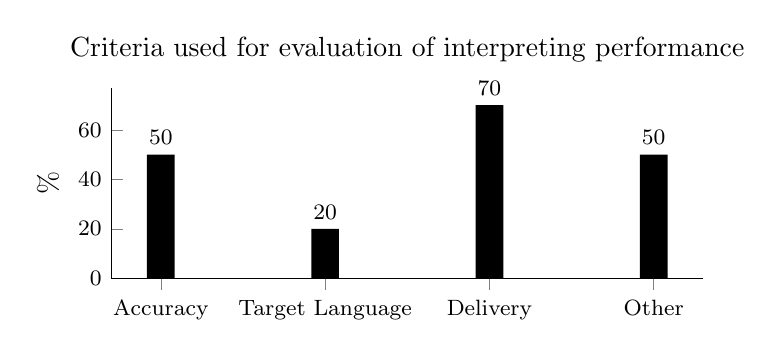
\begin{tikzpicture}
	 \begin{axis}[
	ybar,
	title=Criteria used for evaluation of interpreting performance,
	xtick=data,
	axis lines*=left,
	ymin=0,
	ylabel=\%,
	scaled y ticks=false,
	legend pos=north west,
	reverse legend,
	xticklabels={Accuracy,Target Language,Delivery,Other},
	ticklabel style={font=\footnotesize},
	legend style={font=\footnotesize},
	width=.75\textwidth,
	height=4cm,
	enlarge x limits={0.1},
	nodes near coords,
	nodes near coords style={color=black,font=\footnotesize},
	]
	\addplot+[
	fill=black,draw=none
	] coordinates {(0,50) (1,20) (2,70) (3,50)};
	\end{axis}
	\end{tikzpicture}
\caption{\label{fig:deysel:2}Distribution of perceptions of respondents on criteria\todo[inline]{do we need both caption and plot title?}}
\end{figure}

The data collected and analyzed for the macro error of accuracy indicate that it is the perception of half of the respondents (50\%) that accuracy is important in the evaluation of interpreting performance. The terms “accuracy”, “content accuracy” and “message accuracy” were used. None of the respondents list “omissions” or “additions” as criteria. There were also no examples given of what constitutes “accuracy”.  

The data analyzed for target language indicate that it is the perception of 20\% of respondents that target language is important in the evaluation of interpreting performance. Only two respondents (20\%) listed criteria pertaining to the category of target language by indicating that ‘terminology accuracy’ and ‘vocabulary’ are important criteria in the evaluation of interpreting performance. One respondent (10\%) indicated that ‘sentence construction’ is important when evaluating interpreting performance. 

In the analysis of the data under the macro error of delivery, seven respondents (70\%) listed criteria which pertains to delivery. Eleven different micro errors were listed as criteria important in the evaluation of interpreting performance. The analysis of data gathered from this question reveals a strong focus on the macro error of delivery when seen in relation to the variety of micro errors listed. Two respondents (20\%) listed the micro error pertaining to tone of voice by stating: ‘tone of voice follows the speaker’ and ‘voice tone’. Two respondents (20\%) listed criteria pertaining to the micro error of audibility by listing: ‘audibility’. 

Eleven other micro errors pertaining to the category of delivery were listed; Absence of fillers – 10\%; Avoiding long pauses – 10\%; Breathing – 10\%; Consistency – 10\%; Coherence – 10\%; Correct intonation – 10\%; Delivery smooth and clear – 10\%; Pleasant to hear presentation – 10\%; Time lag 10\%. Only one respondent (10\%) listed criteria across all three different macro errors (accuracy, target language, delivery).

In the qualitative data from the interviews, it was the perception of all respondents that the exposure to the self-assessment sessions had improved their understanding of the criteria used in the evaluation of an interpreting performance. In answer to Q6 (\textit{Before the self-study sessions – were you aware of criteria used in the evaluation of interpreting?)}, two of the respondents indicated that, before the self-assessment sessions, they were not aware of the criteria used in the evaluation of interpreting. Three respondents indicated that they were aware of the criteria used in the evaluation of interpreting. In answer to Q7 (\textit{Do you feel that your understanding of the criteria has improved with the self-study sessions?)} when asked if the respondents’ understanding of the criteria had improved with the exposure to the self-assessment sessions, there was a consensus among all five respondents that their understanding had improved. One respondent indicated that their understanding of the criteria improved, especially after completing the electronic questionnaire. The questions posed in the questionnaire might have triggered the respondents’ thoughts and lead them to reflect on the criteria used when evaluating interpreting performance. The self-assessment grids which were used in the self-assessment session also clearly indicated the various macro errors and criteria used for the evaluation of an interpreting session. 

\section{Conclusion}

One need to emphasize that the study did not seek to evaluate the performance of the interpreters but it was rather aimed at evaluating self-assessment skills of the interpreters. The marks from both the self-assessment and expert ratings were relatively high -  indicating that the interpreters perform at a high level. This ought to be expected since the interpreters are no longer student interpreters, but full-time professional interpreters. The means (both the self-ratings and the ratings by the experts) between the final sessions from the experimental group and the control group did indicate a difference in the averages from the groups (see \tabref{tab:deysel:5}), with the experimental group scoring higher ratings. This indicates that their self-assessment did differ from that of the control group. However, there are several variables which may have contributed to this difference in ratings.  

The empirical study sought to obtain quantitative and qualitative data. The primary research aim of the study set out to evaluate whether the \textsc{CAIT} tool, \textit{Black Box,} was effective in the development of self-assessment skills in professional interpreters. The primary research aim was sub-divided into four research questions and that was covered addressed above under the results. According to the results of this small scale research study, it can be concluded that the \textsc{CAIT} tool, \textit{Black Box,} may prove effective in the development of self-assessment skills in professional interpreters. 


\section*{Addendum A: An example of the self-assessment grid}
\label{03:addendum:A}
\begin{tabularx}{\textwidth}{|XXXXXXXXXXXXXXXXXXXXXXXXXXXXXX|}
\lsptoprule
\rowcolor{lsLightGray}
\multicolumn{30}{p{\textwidth}}{\textbf{SELF-ASSESSMENT SHEET}}\\ \midrule
\multicolumn{30}{p{\textwidth}}{\textbf{Debate on the State of the Nation Address}}\\
\multicolumn{30}{p{\textwidth}}{\textbf{Duration: 6:35min}}\\\midrule
\multicolumn{30}{p{\textwidth}}{Read through all the questions in this self-assessment sheet before you start with the playback of the recording. You are allowed to pause, rewind and make notes while listening to the recording.} \\\midrule
\multicolumn{30}{p{\linewidth}}{PARTICIPANT CODE:}\\ \midrule

\rowcolor{lsLightGray}
\multicolumn{20}{p{0.67\textwidth}}{\textbf{1. ACCURACY / CONTENT OF MESSAGE:}} & \multicolumn{2}{p{0.067\textwidth}}{1} & \multicolumn{2}{p{0.067\textwidth}}{2} & \multicolumn{2}{p{0.067\textwidth}}{3} & \multicolumn{2}{p{0.067\textwidth}}{4} & \multicolumn{2}{p{0.067\textwidth}}{5} \\

\multicolumn{20}{p{0.67\textwidth}}{Omissions, Additions, Accuracy
\textit{The interpreter must convey the message in a complete, correct and intelligible manner in the target language.}} & \multicolumn{2}{p{0.067\textwidth}}{} & \multicolumn{2}{p{0.067\textwidth}}{} & \multicolumn{2}{p{0.067\textwidth}}{} & \multicolumn{2}{p{0.067\textwidth}}{} & \multicolumn{2}{p{0.067\textwidth}}{} \\ \midrule

\multicolumn{2}{p{0.066\textwidth}}{1.1} & \multicolumn{17}{p{0.567\textwidth}}{Was important information omitted in this interpreting session?} & \multicolumn{5}{p{0.167\textwidth}}{YES} & \multicolumn{5}{p{0.167\textwidth}}{NO} \\
\midrule

\rowcolor{lsLightGray}
\multicolumn{20}{p{0.67\textwidth}}{\textbf{2. TARGET LANGUAGE}} & \multicolumn{2}{p{0.067\textwidth}}{1} & \multicolumn{2}{p{0.067\textwidth}}{2} & \multicolumn{2}{p{0.067\textwidth}}{3} & \multicolumn{2}{p{0.067\textwidth}}{4} & \multicolumn{2}{p{0.067\textwidth}}{5} \\

\multicolumn{20}{p{0.67\textwidth}}{Vocabulary, Sentence Construction, Idiomatic language use, Grammar \textit{The interpreter must always use the most appropriate vocabulary and be loyal to the register of the speaker.}} & \multicolumn{2}{p{0.067\textwidth}}{} & \multicolumn{2}{p{0.067\textwidth}}{} & \multicolumn{2}{p{0.067\textwidth}}{} & \multicolumn{2}{p{0.067\textwidth}}{} & \multicolumn{2}{p{0.067\textwidth}}{} \\ \midrule


\multicolumn{2}{p{0.066\textwidth}}{2.1} & \multicolumn{27}{p{0.9\textwidth}}{The following idiomatic language was used in the speech \begin{itemize}
\item write down how each statement was interpreted \item comment on whether the phrase was interpreted into idiomatic target language\end{itemize}} \\
\midrule

\multicolumn{2}{p{0.066\textwidth}}{2.1} & \multicolumn{27}{p{0.9\textwidth}}{[00:20mins] ``\textbf{anxious coin tossing}''}\\
\midrule

\multicolumn{2}{p{0.066\textwidth}}{2.1} & \multicolumn{27}{p{0.9\textwidth}}{[1:40mins] ``He spoke a lot today about iron and steel. Well, let me tell you something: When it comes to the ANC, \textbf{they iron over the problems and steal all the money}.''} \\
\midrule

\rowcolor{lsLightGray}
\multicolumn{20}{p{0.67\textwidth}}{\textbf{3. DELIVERY / COHERENCE / TECHNIQUES and PRESENTATION}} & \multicolumn{2}{p{0.067\textwidth}}{1} & \multicolumn{2}{p{0.067\textwidth}}{2} & \multicolumn{2}{p{0.067\textwidth}}{3} & \multicolumn{2}{p{0.067\textwidth}}{4} & \multicolumn{2}{p{0.067\textwidth}}{5} \\

\multicolumn{20}{p{0.67\textwidth}}{Inarticulate speech, Pauses and hesitations, Audibility, Fillers \textit{The interpreter must maintain sufficient speed to convey the full message of the speaker, employing mechanisms to cope with various complexities, remaining clear and concise.}} & \multicolumn{2}{p{0.067\textwidth}}{} & \multicolumn{2}{p{0.067\textwidth}}{} & \multicolumn{2}{p{0.067\textwidth}}{} & \multicolumn{2}{p{0.067\textwidth}}{} & \multicolumn{2}{p{0.067\textwidth}}{} \\ \midrule

\multicolumn{1}{p{0.033\textwidth}}{3.1} & \multicolumn{18}{p{0.6\textwidth}}{Is the interpreting audible / clear?} & \multicolumn{5}{p{0.167\textwidth}}{YES} & \multicolumn{5}{p{0.167\textwidth}}{NO} \\
\midrule

\multicolumn{1}{p{0.033\textwidth}}{3.2} & \multicolumn{18}{p{0.633\textwidth}}{Are there any fillers (uhm, ah)?} & \multicolumn{5}{p{0.167\textwidth}}{YES} & \multicolumn{5}{p{0.167\textwidth}}{NO} \\
\midrule

\multicolumn{1}{p{0.033\textwidth}}{3.3} & \multicolumn{18}{p{0.633\textwidth}}{Are there any unfinished sentences?} & \multicolumn{5}{p{0.167\textwidth}}{YES} & \multicolumn{5}{p{0.167\textwidth}}{NO} \\
\midrule

\multicolumn{1}{p{0.033\textwidth}}{3.4} & \multicolumn{18}{p{0.633\textwidth}}{Are there any strange noises (coughing, sighing, heavy breathing)?} & \multicolumn{5}{p{0.167\textwidth}}{YES} & \multicolumn{5}{p{0.167\textwidth}}{NO} \\
\midrule

\multicolumn{1}{p{0.033\textwidth}}{3.5} & \multicolumn{18}{p{0.633\textwidth}}{Is the intonation natural or monotonous?} & \multicolumn{5}{p{0.167\textwidth}}{NATURAL} & \multicolumn{5}{p{0.167\textwidth}}{MONOTONOUS} \\
\midrule

\multicolumn{1}{p{0.033\textwidth}}{3.6} & \multicolumn{18}{p{0.633\textwidth}}{Is the lag-time managed well?} & \multicolumn{5}{p{0.167\textwidth}}{YES} & \multicolumn{5}{p{0.167\textwidth}}{NO} \\
\midrule


\rowcolor{lsLightGray}
\multicolumn{20}{p{0.667\textwidth}}{\textbf{TOTAL MARK:}} & \multicolumn{5}{p{0.167\textwidth}}{} & \multicolumn{5}{p{0.167\textwidth}}{\textbf{15}} \\
\lspbottomrule
\end{tabularx}

\section*{Addendum B: Questionnaire}
\label{03:addendum:B}
\begin{tabularx}{\textwidth}{X}
\lsptoprule

\textbf{INTERPRETING QUESTIONNAIRE}\\
\\
Thank you for taking part in this study! This questionnaire is completed anonymously. \\
\lspbottomrule
\end{tabularx}
\begin{tabularx}{\textwidth}{XXXXXXXXXX}
\lsptoprule

\multicolumn{10}{X}{\textbf{Section A: Interpreting Experience}

}\\
&  &  &  &  &  &  &  &  & \\
1 & \multicolumn{9}{X}{In what language(s) do you provide interpreting?

}\\
2 & \multicolumn{9}{X}{How many years’ experience do you have as an interpreter?}\\
& \multicolumn{2}{X}{21 + years

} & \multicolumn{2}{X}{10-20 years} & \multicolumn{2}{X}{5-9 Years} & \multicolumn{3}{X}{Less than 5 years}\\
3 & \multicolumn{9}{X}{How long have you been employed as an interpreter in Parliament?}\\
& \multicolumn{2}{X}{21 + years

} & \multicolumn{2}{X}{10-20 years} & \multicolumn{2}{X}{5-9 Years} & \multicolumn{3}{X}{Less than 5 years}\\
\hhline{~---------}
4 & \multicolumn{6}{X}{Did you have experience in interpreting before you started working at Parliament?} & \multicolumn{2}{X}{YES} & NO\\
5 & \multicolumn{9}{X}{If yes, please specify where you have rendered interpreting services (example; court, clinic, any other):

}\\
6 & \multicolumn{6}{X}{Do you hold a qualification in interpreting/ translation or language practice?} & \multicolumn{2}{X}{YES} & NO\\
7 & \multicolumn{9}{X}{If yes, what qualification do you hold?}\\
& \multicolumn{1}{X}{Diploma

} & \multicolumn{2}{X}{Bachelors} & \multicolumn{2}{X}{Honours} & \multicolumn{2}{X}{Masters} & \multicolumn{2}{X}{PhD}\\
\hhline{~---------} & \multicolumn{9}{X}{Other, specify:}\\
8 & \multicolumn{6}{X}{Have you received any informal interpreter training?} & \multicolumn{2}{X}{YES} & NO\\
9 & \multicolumn{9}{X}{If yes, please specify what type of training you received (example; short courses, in-house training, any other):}\\
\lspbottomrule
\end{tabularx}
\begin{tabularx}{\textwidth}{XXXXXXX}
\lsptoprule

\multicolumn{7}{X}{\textbf{Section B: Self-assessment activities}

}\\
&  &  &  &  &  & \\
10 & \multicolumn{6}{X}{How often do you:}\\
&  & Never & Seldom & Frequently & Always & N/A\\
10.1 & Record your interpreting sessions &  &  &  &  & \\
10.2 & Listen to recordings of your interpreting sessions &  &  &  &  & \\
10.3 & Take note of terminology which is challenging in an interpreting session &  &  &  &  & \\
10.4 & Take note of challenges presented in an interpreting session &  &  &  &  & \\
10.5 & Conduct self-assessment on an interpreting performance &  &  &  &  & \\
\lspbottomrule
\end{tabularx}
\begin{tabularx}{\textwidth}{XXXXXXX}
\lsptoprule

\multicolumn{7}{X}{\textbf{Section C: Interpreting strengths and weaknesses}

}\\
&  &  &  &  &  & \\
11 & \multicolumn{6}{X}{How often do you struggle with the following challenges in interpreting?

}\\
&  & Never & Seldom & Frequently & Always & N/A\\
11.1 & Interpreting proper names &  &  &  &  & \\
11.2 & Interpreting numbers and figures &  &  &  &  & \\
11.3 & Interpreting dates &  &  &  &  & \\
11.4 & Understanding the speakers’ accent &  &  &  &  & \\
11.5 & Following the speakers’ speed &  &  &  &  & \\
\multicolumn{7}{X}{}\\
12 & \multicolumn{6}{X}{Indicate your ability with regards to the following in simultaneous interpreting:

}\\
&  & Never & Seldom & Frequently & Always & N/A\\
12.1 & I struggle to provide an accurate message &  &  &  &  & \\
12.2 & I pause within the middle of a sentence &  &  &  &  & \\
12.3 & I struggle with target language register &  &  &  &  & \\
12.4 & I struggle with target language terminology &  &  &  &  & \\
12.5 & I hesitate &  &  &  &  & \\
12.6 & I have a monotonous intonation &  &  &  &  & \\
12.7 & I use filler words such as \textit{uhm} and a\textit{h} within a sentence &  &  &  &  & \\
12.8 & My speech is unclear &  &  &  &  & \\
12.9 & I struggle with target language grammar &  &  &  &  & \\
12.10 & My target language use is unidiomatic &  &  &  &  & \\
12.11 & I omit information &  &  &  &  & \\
12.12 & I add information &  &  &  &  & \\
12.13 & I do not finish sentences &  &  &  &  & \\
12.14 & My message delivery is incoherent &  &  &  &  & \\
12.15 & I struggle with microphone use &  &  &  &  & \\
12.16 & I need to improve my simultaneous interpreting technique &  &  &  &  & \\
12.17 & I struggle to concentrate while interpreting &  &  &  &  & \\
12.18 & I speak too fast &  &  &  &  & \\
12.19 & I breathe loud &  &  &  &  & \\
12.20 & I get emotionally involved &  &  &  &  & \\
12.21 & My delivery is smooth and flows with ease &  &  &  &  & \\
12.22 & I convey the message accurately &  &  &  &  & \\
12.23 & I do not make irritating noises &  &  &  &  & \\
12.24 & My voice sounds pleasant &  &  &  &  & \\
12.25 & I use the appropriate terminology &  &  &  &  & \\
12.26 & I do not stop in the middle of a sentence &  &  &  &  & \\
\lspbottomrule
\end{tabularx}
\begin{tabularx}{\textwidth}{XX}
\lsptoprule

\multicolumn{2}{X}{\textbf{Section D: Evaluation of Interpreting Performance}

}\\
& \\
13 & List the criteria which you find important in the evaluation of an interpreting performance:\\
14 & Define each of the following macro errors when used to evaluate interpreting performance:\\
14.1 & Accuracy\\
14.2 & Delivery\\
14.3 & Target Language Quality\\
15 & Provide examples of errors according to the following macro errors (for example; accuracy = omissions):\\
15.1 & Accuracy\\
15.2 & Delivery\\
15.3 & Target Language Quality\\
16 & Do you have any other comments?\\
\lspbottomrule
\end{tabularx}

\section*{Addendum C: Interview questions}
\label{03:addendum:C}
\begin{description}
\item[Q1:] Was this the first time you recorded your interpreting performance?
\item[Q2:] Was this the first time you listened to yourself interpreting?
\item[Q3:] Were you satisfied with your interpreting performance? 
\item[Q4:] Was your interpreting performance better or worse than you expected?
\item[Q5:] In the questionnaire there was a section pertaining to your abilities in interpreting. After having conducted self-assessment – do you think that your initial judgements were correct?
\item[Q6:] Before the self-study sessions – were you aware of criteria used in the evaluation of interpreting?
\item[Q7:] Do you feel that your understanding of the criteria has improved with the self-study sessions?
\item[Q8:] In your first self-study session and self-assessment did you find it difficult to assess yourself?
\item[Q9:] Do you feel that the self-study sessions have developed your self-assessment skills?
\item[Q10:] Do you feel that it is easier being assessed on your interpreting performance by someone else?
\item[Q11:] Do you think that if someone was to assess this very same assessment that you would receive the very same mark?
\item[Q12:] Did you find the self-study sessions useful in order to conduct self-assessment?
\item[Q13:] Did you find the self-assessment grids useful in your self-assessment?
\item[Q14:] Do you feel that the self-study sessions have given you a better awareness of your strengths and weaknesses in interpreting?
\item[Q15:] Do you feel that the self-study sessions have improved your interpreting performance?
\item[Q16:] What did you find most useful in the self-study sessions?
\item[Q17:] Do you feel that the self-study sessions have made you more confident in conducting self-assessment on your interpreting performance?
\item[Q18:] Do you have any other comments?
\end{description}
 
\section*{Abbreviations}
\section*{Acknowledgements}

{\sloppy\printbibliography[heading=subbibliography,notkeyword=this]}
\end{document}
